
%=========================================================================
% Start of
%=========================================================================
\preClass{Distance and Circles}

Expand each of the functions below by FOILing the expression. The
first one is done as an example. Recall what it means to FOIL an
expression.

  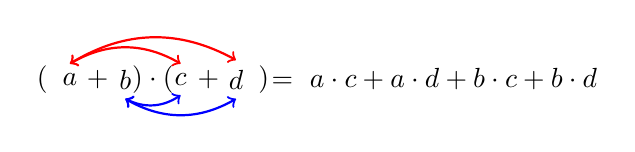
\begin{tikzpicture}[y=1em, x=1em,font=\sffamily]
    %% Draw the (a+b) part
    \node     at (0,0) {$($};
    \node (a) at (1,0) {$a$};
    \node     at (2,0) {$+$};
    \node (b) at (3,0) {$b$};
    \node     at (4,0) {$)\cdot($};

    %% Draw the *(c+d) part
    \node (c) at (5,0) {$c$};
    \node     at (6,0) {$+$};
    \node (d) at (7,0) {$d$};
    \node     at (8,0) {$)$};

    %% Draw the right hand side of the equation
    \node     at (14,0) {$~=~a\cdot c + a\cdot d + b\cdot c + b\cdot d$};

    %% Now make the pretty lines between the parts to FOIL
    \path[red,<->,thick] (a.north) edge[bend left] node {} (c.north);
    \path[red,<->,thick] (a.north) edge[bend left] node {} (d.north);

    \path[blue,<->,thick] (b.south) edge[bend right] node {} (c.south);
    \path[blue,<->,thick] (b.south) edge[bend right] node {} (d.south);

  \end{tikzpicture}


\begin{problem}
\item ${\displaystyle (x-3)^2}$

  Answer:
  \begin{eqnarray*}
    (x-3) & = & (x-3)\cdot(x-3), \\
    & = & x\cdot x - 3\cdot x - 3\cdot x + (-3)\cdot(-3), \\
    & = & x^2 - 3x - 3x + 9, \\
    & = & x^2 - 6x + 9.
  \end{eqnarray*}
\item ${\displaystyle }$
  \vfill
\item ${\displaystyle }$
  \vfill
\item ${\displaystyle }$
  \vfill
\end{problem}


\actTitle{Graphs of Equations}
\begin{problem}
\item Sketch a graph of the relationship given by
  \begin{eqnarray*}
    x^2 + 2x + y^2 - 8y & = & 8.
  \end{eqnarray*}
  Determine the center and the radius of the circle.
  Make a sketch of the circle. (Label the axes.)
  \vfill

  \clearpage

\item Windows are constructed, and their width is proportional to
  their height. One window is measured, and its width is 100cm, and its
  height is 200cm. Make a sketch of the relationship of the height of
  a window given its width. Briefly discuss the relationship. How does
  the height change as the width changes?
  \sideNote{Annotate your plot and label your axes!}

  \vfill

\item The surface area of a sparrow's wing is proportional to the
  square of the length of its wing. A sparrow is measured, and it has
  a wing length of 9cm and an area of 45cm\textsuperscript{2}. Make a
  sketch of the relationship of the area of a sparrow's wing given the
  length. Briefly discuss the relationship. How does the area change
  as the length changes?
  \sideNote{Annotate your plot and label your axes!}

  \vfill

\clearpage

\item The mass of a sparrow is proportional to the cube of the length of its wing.
  \begin{subproblem}
    \item \label{sparrowWingArea} A sparrow is measured, and it has a wing length of 9cm and a mass of 30 grams.
    Determine the mass of a sparrow whose wing length is 10cm.
    \vfill

    \item \label{sparrowMass} It is estimated that the mass of a sparrow is 27 grams. Determine an estimate
    of its wing length.
    \vfill
  \end{subproblem}

\end{problem}

\postClass

\begin{problem}
\item Briefly state two ideas from today's class.
  \begin{itemize}
  \item
  \item
  \end{itemize}
\item A circle is circumscribed within a square so it just touches on
  each of the four edges of the square.
  \begin{subproblem}
    \item Make a sketch of the square and circle. Mark the length of
      the square and the radius of the circle.
    \item Determine the relationships between the length of the edge,
      the radius of the circle, the area of the square, and the area
      of the circle.
    \item Determine the area of the square not covered by the circle
      as a function of the length of one side of the square.
    \item Make a sketch of a graph of the area of the square not
      covered by the circle. The horizontal axis should be the length
      of one side of the square, and the vertical axis should be the
      area. Label your axes.
    \item How does the area change as the length of one side of the
      square increases? (Does it change linearly, does the rate of
      change increase or decrease?)
    \item Determine the proportion of the area not covered by the
      circle with respect to the area of the square. What percentage
      of the area of the square is not covered? How does this change
      as the length of one side of the square changes?
  \end{subproblem}
  \item You watch a video from your favourite conspiracy theorist.
    He says that scientists are supressing evidence about prehistoric sparrows.
    He says that giant sparrows once existed whose wing length was 10 meters.
    Use the results from exercises  \ref{sparrowWingArea} and \ref{sparrowMass} to determine if this makes sense.
    Based on your result write out the comment that you will post in the comments
    section in response to the video.

\end{problem}



%%% Local Variables:
%%% mode: latex
%%% TeX-master: "functions"
%%% End:
